\documentclass[aspectratio=169]{beamer}
\usetheme[block=fill]{metropolis}
\usepackage{tikz}
\usetikzlibrary{shapes.geometric, arrows.meta, positioning, calc}

\title{Building a Reproducible Scholarly Search Toolkit}
\subtitle{Episode 16: Pluggable Output Formats (JSONL \& RIS)}
\author{Scholar Search Kit}
\date{}

\begin{document}

\begin{frame}[plain]
  \titlepage
\end{frame}

\begin{frame}{Episode Goal}
  \begin{alertblock}{The Goal}
    Create a serialization subsystem that can write our \texttt{Document} models to disk in various academic formats.
  \end{alertblock}
  \vspace{0.5cm}
  Developers want JSONL. Researchers want RIS so they can drag-and-drop into Zotero or Mendeley. Our tool must support both.
\end{frame}

\begin{frame}{The \texttt{Exporter} Protocol}
  \begin{center}
  \resizebox{0.5\linewidth}{!}{
  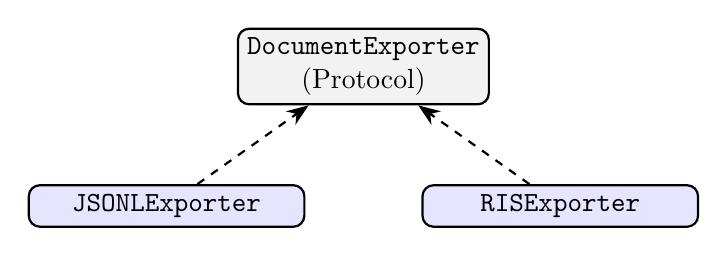
\begin{tikzpicture}[
      node distance=1.5cm and 2cm,
      proto/.style={rectangle, draw, thick, rounded corners, minimum width=3cm, align=center, fill=black!5},
      impl/.style={rectangle, draw, thick, rounded corners, minimum width=3.5cm, align=center, fill=blue!10},
      arrow/.style={-{Stealth[scale=1.2]}, thick, dashed}
    ]
    
    \node[proto] (p) {\texttt{DocumentExporter}\\(Protocol)};
    
    \node[impl, below=1cm of p, xshift=-2.5cm] (json) {\texttt{JSONLExporter}};
    \node[impl, below=1cm of p, xshift=2.5cm] (ris) {\texttt{RISExporter}};
    
    \draw[arrow] (json) -- (p);
    \draw[arrow] (ris) -- (p);
  \end{tikzpicture}
  }
  \end{center}
  \vspace{0.2cm}
  Every exporter implements \texttt{write\_chunk(docs: list[Document])}.
\end{frame}

\begin{frame}{Implementation: JSON Lines (JSONL)}
  \begin{block}{Machine Readable}
    JSONL puts one complete JSON object per line.
  \end{block}
  
  \begin{itemize}
      \item Perfect for streaming. You can append to the file without breaking syntax (unlike standard JSON arrays).
      \item Easy to ingest into Pandas or BigQuery.
  \end{itemize}
\end{frame}

\begin{frame}{Implementation: RIS Format}
  \begin{block}{The Academic Standard}
    RIS uses two-letter tags (e.g., \texttt{TI  - Title}, \texttt{AU  - Author}).
  \end{block}
  
  \begin{itemize}
      \item Requires careful formatting. Every tag must be separated by exactly two spaces and a hyphen.
      \item \texttt{ER  - } marks the end of a record.
  \end{itemize}
\end{frame}

\begin{frame}{Verification}
  \begin{alertblock}{Success Criteria}
    \begin{itemize}
        \item The \texttt{JSONLExporter} produces valid JSON that \texttt{json.loads()} can read.
        \item The \texttt{RISExporter} produces a text file that a citation manager (or our mock parser) can successfully import.
    \end{itemize}
  \end{alertblock}
\end{frame}

\end{document}
